\section{Alati}

\subsection{Apstraktna sintaksna stabla}
Apstraktno sintaksno stablo (eng.\ \textsl{abstract syntax tree}, \textsl{AST}) je struktura podataka koja predstavlja strukturu programskog koda u nekom programskom jeziku. Vrhovi tog stabla odgovaraju sintaktičkim konstruktima u jeziku. Primjerice, vrh može odgovarati binarnoj operaciji. U tom slučaju lijevo i desno podstablo odgovaraju operandima, koji, rekurzivno, sami mogu imati više binarnih operacija u sebi. Vrh može odgovarati for-petlji --- tada su sva djeca podstabla koja odgovaraju konstruktima unutar bloka određenog for-petljom. Ostali važni podaci, kao što su varijabla i granice iteracije, mogu biti spremljeni kao atributi tog objekta ili ponovo kao djeca glavnog vrha.

Apstraktna sintaksna stabla su međukorak prilikom kompilacije programskog koda u većini modernih programskih jezika. Tako i Pythonov kompajler stvara AST prije eventualnog prijevoda u \emph{bytecode}. Apstraktna sintaksna stabla su dio samog kompajlera, ali modul \texttt{ast.py} (službena dokumentacija pod~\cite{docs:ast}, podrobnija dokumentacija pod~\cite{docs:gts}) u standardnoj biblioteci služi kao omotač koji nudi AST kao objekt u Pythonu s nekoliko pomoćnih funkcija za njihovu obradu.

Postojeće funkcionalnosti modula \texttt{ast.py} dozvoljavaju pregled stabla u formatu sličnom JSON-u (\texttt{ast.dump}), ali pomoću paketa Graphviz ih možemo vizualizirati grafički. Razmotrimo sljedeći isječak koda:
\begin{lstlisting}[language=Python]
x = 1
class A:
    def __init__(self, x=5):
        self.x = x

a = A()
\end{lstlisting}
Odgovarajuće apstraktno sintaksno stablo dano je na slici~\ref{fig:ast-example}.
Tekst u čvorovima odgovara različitim klasama u modulu, potklasama bazne klase \texttt{ast.AST} (npr.\ \texttt{ast.ClassDef} odgovara definiranju klase), a dodatne informacije, kao što je ime objekta ili vrijednost konstante, dane su ispod.
Najčešće, čvorovi imaju još relevantnih atributa, ali na slici nisu prikazani u svrhu preglednosti.

% caption vs ref
\begin{figure}[hb]
    \centering
    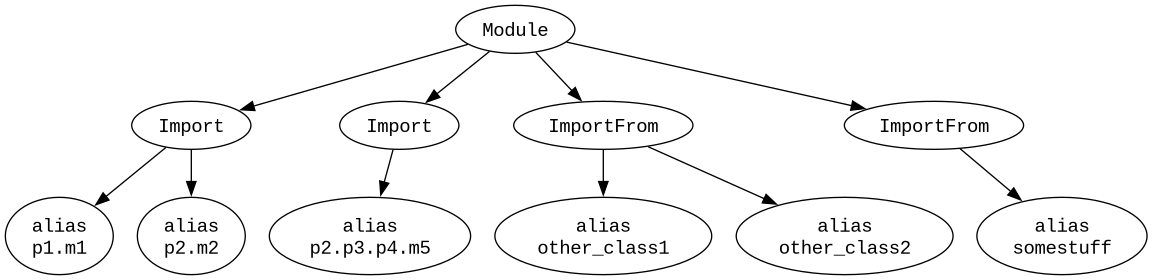
\includegraphics[width=0.5\textwidth]{assets/ast-example.png}
    \caption{Primjer AST-a}
    \label{fig:ast-example}
\end{figure}

\subsection{Tablice simbola}
Tablica simbola (eng.\ \textsl{symbol table}) je još jedna struktura podataka koju koriste kompajleri. Generira se nakon AST-a, te u Pythonovom slučaju direktno prethodi konačnoj kompilaciji. Kao i AST, moguć joj
je pristup kao objektu u Pythonu preko modula \texttt{symtable.py} (službena dokumentacija pod~\cite{docs:symtable}) iz standardne biblioteke. 

Tablica simbola sadrži sve simbole u kodu, a posebno se pritom osvrće na njihove opsege (\emph{scope}-ove) i eventualno neke dodatne atribute. Pritom, glavna tablica sadrži globalni nazivni prostor (\emph{namespace}), 
a može sadržavati i podtablice sa vlastitim, lokalnim nazivnim prostorima. U Pythonu, to je slučaj za nazivne prostore klasa i funkcija, ali ne, za razliku od drugih jezika, for-petlji ili sličnih blokova koje nemaju vlastiti 
nazivni prostor.

Budući da se tablica generira iz samog AST-a, sve što možemo napraviti s tablicama simbola možemo i sa samim AST-om. Ipak, uporaba modula iz standardne biblioteke smanjuje mogućnost greške i osigurava usklađenost s
Pythonovim kompajlerom. Za primjer toga što je sve dostupno u Pythonu, čitatelj može pogledati primjer ispisa u bilježnici
\begin{center}
\texttt{example/symtable_example.ipynb}
\end{center}
u repozitoriju projekta~\cite{repo}.


